\tikzstyle{yes}=[draw, rectangle, fill=green!30,minimum width=3cm, minimum height=0.8cm]
\tikzstyle{no}=[draw, rectangle, fill=yellow!30,minimum width=3cm, minimum height=0.8cm]
\tikzstyle{maybe}=[draw, rectangle, fill=yellow!30,minimum width=3cm, minimum height=0.8cm]

\begin{frame}
\frametitle<1-2>{Classify the Image}
\frametitle<3-4>{Classify the Image}
\frametitle<5->{Classify the Image}
\centering
\resizebox{\textwidth}{!}{
\begin{tikzpicture}
%\tikzstyle{yes}=[draw, rectangle, fill=green!30,minimum width=1in]
%\tikzstyle{no}=[draw, rectangle, fill=yellow!30,minimum width=1in]
%\tikzstyle{maybe}=[draw, rectangle, fill=yellow!30,minimum width=1in]

\uncover<1>{
\node (image) at (0,0.25) {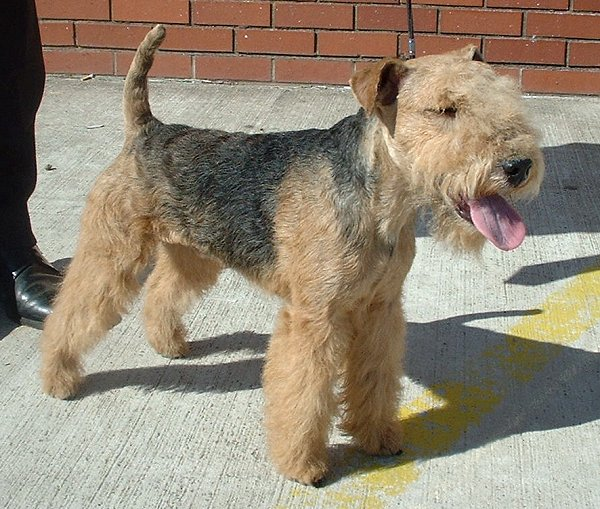
\includegraphics[height=2.25in]{img/Lakeland_Terrier}};
\node[maybe] at (-2,-4) {Animal};
\node[maybe] at (2,-4) {Not-Animal};
}

\uncover<2>{
\node (image) at (0,0.25) {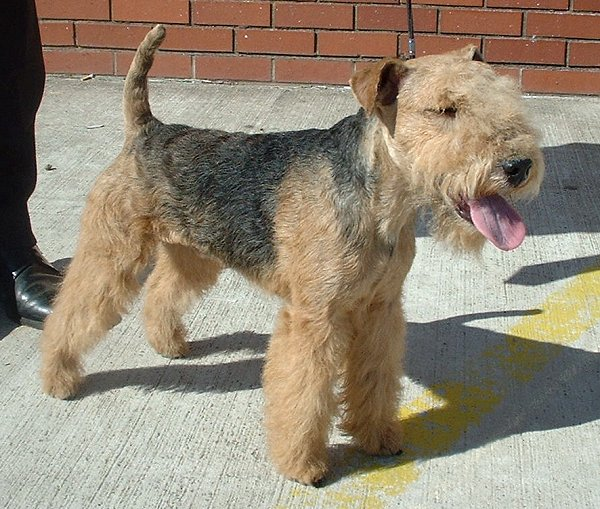
\includegraphics[height=2.25in]{img/Lakeland_Terrier}};
\node[yes] at (-2,-4) {Animal};
\node[maybe] at (2,-4) {Not-Animal};
}

\uncover<3>{
\node (image) at (0,0.25) {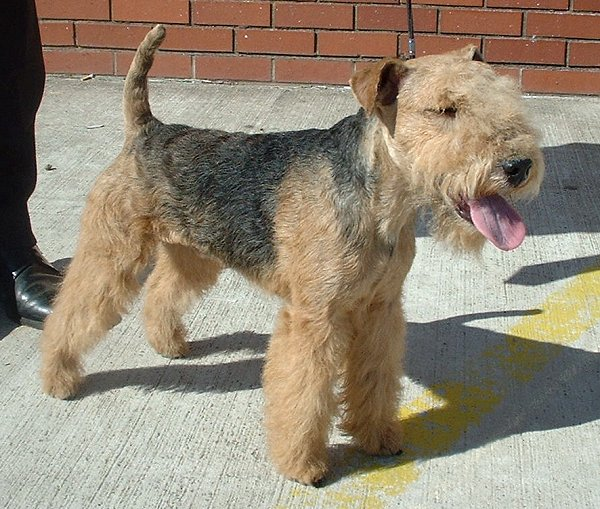
\includegraphics[height=2.25in]{img/Lakeland_Terrier}};
\node at (-3.25,-3) {\footnotesize Animal};
\node at (3.5,-3) {\footnotesize Not-Animal};
\draw (-6.5,-3.325) -- (-0.25, -3.325);
\draw (6.5,-3.325) -- (0.25, -3.325);
\node[maybe] at (-5,-4) {Fish};
\node[maybe] at (-1.6875,-4) {Bird};
\node[maybe] at (1.6875,-4) {Vehicle};
\node[maybe] at (5,-4) {Plant};
\node[maybe] at (-5,-5) {Insect};
\node[maybe] at (-1.6875,-5) {Mammal};
\node[maybe] at (1.6875,-5) {Building};
\node[maybe] at (5,-5) {Object};
}

\uncover<4>{
\node (image) at (0,0.25) {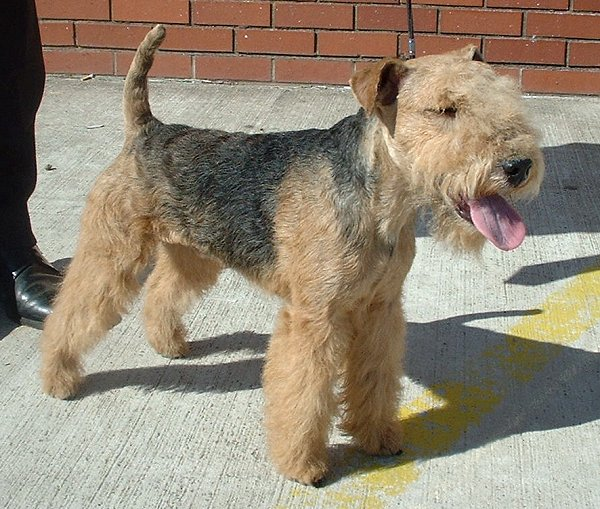
\includegraphics[height=2.25in]{img/Lakeland_Terrier}};
\node at (-3.25,-3) {\footnotesize Animal};
\node at (3.5,-3) {\footnotesize Not-Animal};
\draw (-6.5,-3.325) -- (-0.25, -3.325);
\draw (6.5,-3.325) -- (0.25, -3.325);
\node[maybe] at (-5,-4) {Fish};
\node[maybe] at (-1.6875,-4) {Bird};
\node[maybe] at (1.6875,-4) {Vehicle};
\node[maybe] at (5,-4) {Plant};
\node[maybe] at (-5,-5) {Insect};
\node[yes] at (-1.6875,-5) {Mammal};
\node[maybe] at (1.6875,-5) {Building};
\node[maybe] at (5,-5) {Object};
}

%\uncover<4>{
%\node (image) at (0,0.25) {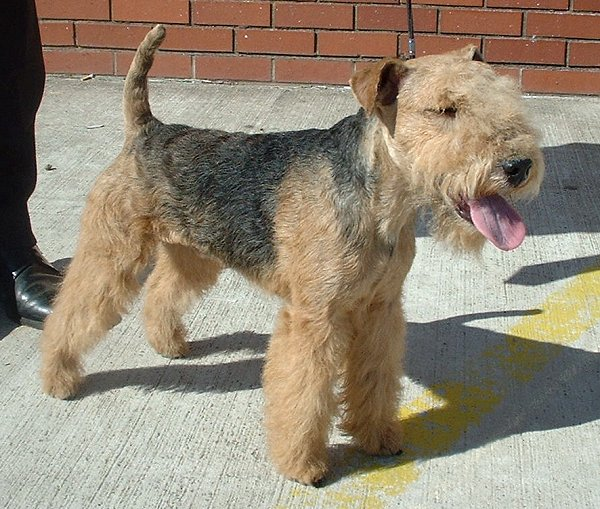
\includegraphics[height=2.25in]{img/Lakeland_Terrier}};
%\node at (-3.25,-3) {\footnotesize Animal};
%\node at (3.5,-3) {\footnotesize Not-Animal};
%\draw (-6.5,-3.325) -- (-0.25, -3.325);
%\draw (6.5,-3.325) -- (0.25, -3.325);
%\node[maybe] at (-5,-4) {Cat};
%\node[yes] at (-1.6875,-4) {Dog};
%\node[maybe] at (1.6875,-4) {Car};
%\node[maybe] at (5,-4) {Tree};
%\node[maybe] at (-5,-5) {Horse};
%\node[maybe] at (-1.6875,-5) {Fish};
%\node[maybe] at (1.6875,-5) {House};
%\node[maybe] at (5,-5) {Hat};
%}

\uncover<5>{
\node (image) at (0,0.25) {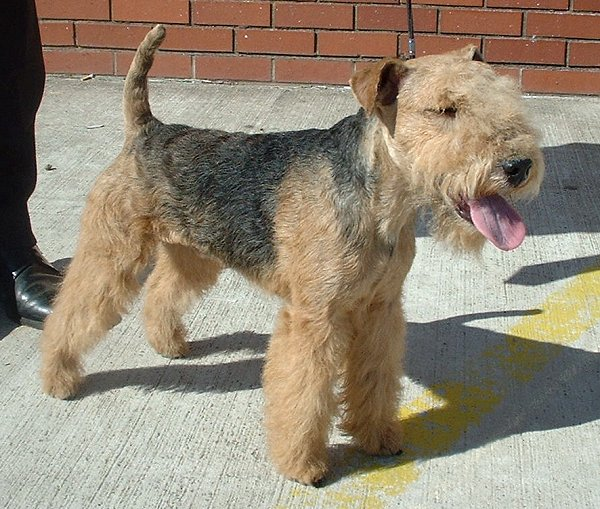
\includegraphics[height=2.25in]{img/Lakeland_Terrier}};
\node at (0,-3.5) {\Large ImageNet has 1000 different classes};
\node at (0,-4.5) {\Large (80 different dog breeds)};
    %\node at (0,-5) {\Large generalization error = $O(\sqrt{k/n})$};
}

\uncover<6>{
\node (image) at (0,0.25) {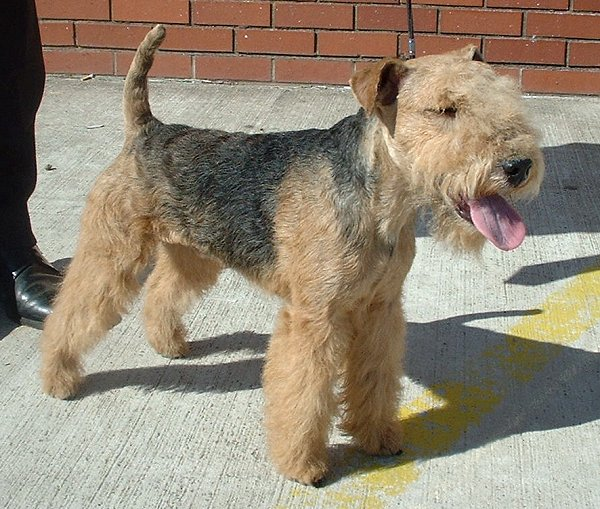
\includegraphics[height=2.25in]{img/Lakeland_Terrier}};
\node[maybe] at (-5,-4) {Irish Terrier};
\node[maybe] at (-1.6875,-4) {Airedale};
%\node[maybe] at (1.6875,-4) {Horse};
%\node[maybe] at (5,-4) {Human};
\node[maybe] at (-5,-5) {Lakeland Terrier};
\node[maybe] at (-1.6875,-5) {Irish Spaniel};
%\node[maybe] at (1.6875,-5) {House};
%\node[maybe] at (5,-5) {Hat};
\node at (3.5,-4.5) {Note shown: 996 other classes};
}

\uncover<7>{
\node (image) at (0,0.25) {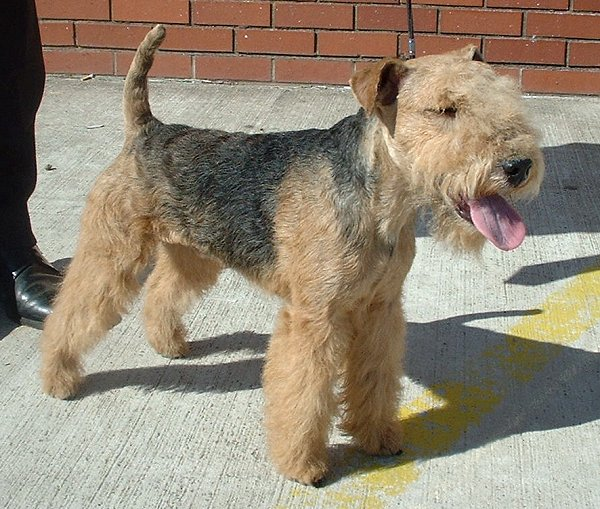
\includegraphics[height=2.25in]{img/Lakeland_Terrier}};
\node[maybe] at (-5,-4) {Irish Terrier};
\node[maybe] at (-1.6875,-4) {Airedale};
\node[yes] at (-5,-5) {Lakeland Terrier};
\node[maybe] at (-1.6875,-5) {Irish Spaniel};
\node at (3.5,-4.5) {Note shown: 996 other classes};
}

\uncover<8>{
\node (image) at (0,0.25) {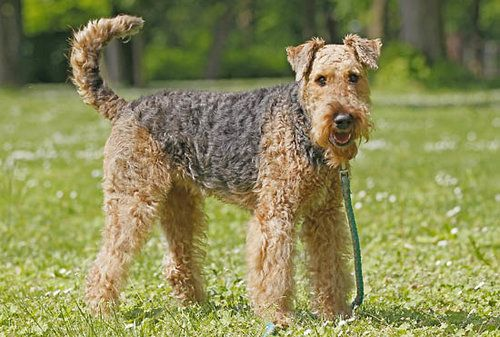
\includegraphics[height=2.25in]{img/Airedale}};
\node[maybe] at (-5,-4) {Irish Terrier};
\node[yes] at (-1.6875,-4) {Airedale};
\node[maybe] at (-5,-5) {Lakeland Terrier};
\node[maybe] at (-1.6875,-5) {Irish Spaniel};
\node at (3.5,-4.5) {Note shown: 996 other classes};
}

\uncover<9>{
\node (image) at (0,0.25) {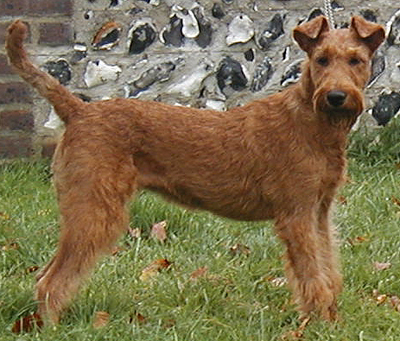
\includegraphics[height=2.25in]{img/Irish-Terrier}};
\node[yes] at (-5,-4) {Irish Terrier};
\node[maybe] at (-1.6875,-4) {Airedale};
\node[maybe] at (-5,-5) {Lakeland Terrier};
\node[maybe] at (-1.6875,-5) {Irish Spaniel};
\node at (3.5,-4.5) {Note shown: 996 other classes};
}

\uncover<10>{
\node (image) at (0,0.25) {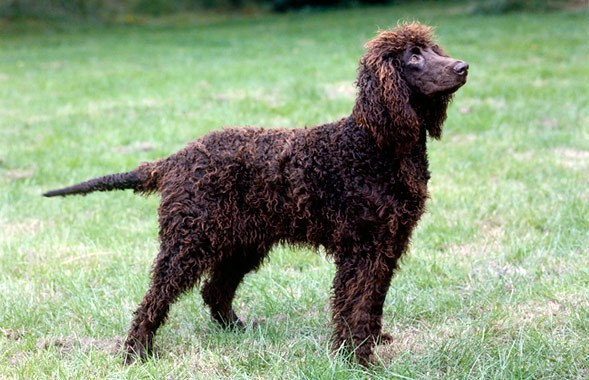
\includegraphics[height=2.25in]{img/water_spaniel}};
\node[maybe] at (-5,-4) {Irish Terrier};
\node[maybe] at (-1.6875,-4) {Airedale};
\node[maybe] at (-5,-5) {Lakeland Terrier};
\node[yes] at (-1.6875,-5) {Irish Spaniel};
\node at (3.5,-4.5) {Note shown: 996 other classes};
}

%\uncover<11> {
    %\node at (0, 2) {\Large more classes $\Rightarrow$ harder problem};
%
    %\node at (0, 0) {\Large real world problems are highly structured };
%
    %\node at (0, -2) {\Large \textbf{This talk:} exploit class structure to make the problem easier};
%}

\end{tikzpicture}
}
\end{frame}

%%%%%%%%%%%%%%%%%%%%%%%%%%%%%%%%%%%%%%%%%%%%%%%%%%%%%%%%%%%%%%%%%%%%%%%%%%%%%%%%

\ignore{
\begin{frame}
\frametitle{(Informal) Main Idea}

%ImageNet: 1000 classes, 80 breeds of dogs

Classification gets ``harder'' when we
\begin{itemize}
\item add more classes
\item the classes are ``more similar''
\end{itemize}

\vspace{0.2in}
This talk:
\begin{itemize}
\item formalize ``harder'' (machine learning)
\item formalize ``more similar'' (discrete geometry)
\item fix the problem
\end{itemize}

\end{frame}
}
